%%%
%
% $Autor: Vikas Ramaswamy$
% $Datum: 2023-03-17 11:15:45Z $
% $Pfad: GitLab/CornerBlending $
% $Dateiname: ArcStrategy
% $Version: 4620 $
%
% !TeX spellcheck = de_GB
%
%%%






\chapter{Development}

Before any actual implementation, a number of subprocesses that are relevant to each project's goals must be understood and defined in order for the KDD methodology to be used in a practical way. To gain a deeper understanding of the project's data environment, we will discuss the database. The purpose of this chapter is to discuss the steps involved in each KDD process as well as how the KDD process is executed. The proposed approach for the workflow is shown in figure 4.1:

%%\begin{tikzpicture}[node distance=2cm]
		% Nodes
%%	\node (start) [draw, rounded rectangle] {Start};
%%	\node (data) [draw, rectangle, below of=start] {Data Collection
	%%	(Pneumonia dataset from Kaggle)};
%%	\node (xray) [draw, rectangle, below of=data] {X-ray Images};
%%	\node (resize) [draw, rectangle, below of=xray] {Resize the images to standard size};
%%	\node (pixel) [draw, rectangle, below of=resize] {The pixel values of  images are normalized};
%%	\node (split) [draw, rectangle, below of=pixel] {Data Splitting};
%%	\node (train) [draw, rectangle, below left of=split, xshift=-1.5cm] {Train};
%%	\node (validate) [draw, rectangle, below of=split] {Validate};
%%	\node (test) [draw, rectangle, below right of=split, xshift=1.5cm] {Test};
%%	\node (train2) [draw, rectangle, below of=train] {Training};
%%	\node (pred) [draw, rectangle, below of=train2] {Predictions};
%%	\node (valid) [draw, rectangle, below of=validate] {Validating Model};
	
%%	\node (detect) [draw, rectangle, below of=valid, xshift=3cm] {Make Detection};
%%	\node (pneumonia) [draw, rounded rectangle, below of=detect, xshift=-2.5cm] {Pneumonia};
%%	\node (normal) [draw, rounded rectangle, below of=detect, xshift=2.5cm] {Normal};
	
%%	% Arrows
%%	\draw [->] (start) -- (data);
%%	\draw [->] (data) -- (xray);
%%	\draw [->] (xray) -- (resize);
%%	\draw [->] (resize) -- (pixel);
%%	\draw [->] (pixel) -- (split);
%%	\draw [->] (split) -- (train);
%%	\draw [->] (split) -- (validate);
%%	\draw [->] (split) -- (test);
%%	\draw [->] (train) -- (train2);
%%	\draw [->] (train2) -- (pred);
%%	\draw [->] (pred) -- (valid);
%%	\draw [->] (validate) -- (valid);
	%%\draw [->] (valid) -- (train2);
	%%\draw [->] (valid) -- (detect);
	%%\draw [->] (test) -- (detect);
	%%\draw [->] (detect) -- (pneumonia);
	%%\draw [->] (detect) -- (normal);
	
%%\end{tikzpicture}

\begin{figure}
	\centering
	\begin{tikzpicture}
		\node at (0,0) {\includegraphics[width=\linewidth]{Images/Pneumonia Detection-2.png}};
	\end{tikzpicture}
	\caption{\textbf{KDD approach flow chart}}
	\footnotesize \textbf{Reference:Author}
	\label{fig:KDD Approach}
\end{figure}

\bigskip

\section{Database Description}

The database used in the project contains chest X-ray images (JPEG) of pediatric patients of one to five years old from Guangzhou Women and Children’s Medical Center, Guangzhou. The dataset is organized into 3 folders train, test, val for training,testing and validating respectively. Further each folder contains subfolders for each image category for Pneumonia and Normal. There are 5,863 X-Ray images (JPEG) and 2 categories (Pneumonia/Normal).\cite{Wang:2017}

 
 \bigskip
 
 \section{Dataset Description}
 
There are 2 categories and 5,863 X-Ray images in JPEG format. The total file is around 2GB in size. From retrospective cohorts of children patients aged one to five at the Guangzhou Women and Children's Medical Center in Guangzhou, chest X-ray images (anterior-posterior) were chosen. All chest X-ray imaging was done as part of the regular clinical treatment provided to patients. All chest radiographs were initially screened for quality control before being removed from the analysis of the chest x-ray images. Before the diagnosis for the photos could be used to train the AI system, they were graded by two experienced doctors. A third expert also reviewed the evaluation set to make sure there were no grading mistakes.

\begin{figure}
	\centering
	\begin{tikzpicture}
		\node at (0,0) {\includegraphics[width=\linewidth]{Images/Dataset sample.png}};
	\end{tikzpicture}
	\caption{\textbf{Chest X-ray of (a) Healthy person and (b) Pneumonia}}
	\footnotesize \textbf{Reference:}\cite{Firdiantika:2022}
	\label{fig:Chest X-ray images of healthy person and person having pneumonia}
\end{figure}

\subsection{Mendeley Chest X-Ray Dataset}

\begin{enumerate}
	\item \textbf{Origin:} The Mendeley Chest X-Ray Dataset was created by a team of researchers from the National Institutes of Health (NIH), Montgomery County, Maryland, USA. It is a public dataset, which was created to aid researchers and developers in the creation of AI algorithms for the detection of pneumonia in chest x-ray images.\autocite{Cohen:2017}

\item \textbf{Features:} The dataset contains 5,856 chest x-ray images in PNG format, out of which 3,955 are normal, and 1,920 have pneumonia. Each image is labeled with the corresponding diagnosis. The dataset also includes a metadata file that contains patient demographics, image modality, and image metadata.\\

\item \textbf{Data Types:} The dataset includes grayscale chest x-ray images in PNG format. The metadata file includes data in various formats, such as integers, strings, and date/time stamps.\\

\item \textbf{Quality:} The quality of the dataset is considered to be high as it is a public dataset created by the NIH, which is a reputable organization. The images were acquired from various sources, including pediatric and general radiology departments, and are of high quality. The metadata is also comprehensive and provides useful information about the images.\\

\item \textbf{Bias:} The dataset has a limited representation of different ethnicities and genders, which may result in bias towards certain groups. Additionally, the dataset primarily includes chest x-ray images from patients with pneumonia, which may result in an imbalance between normal and abnormal cases.\\

\end{enumerate}

\subsection{Kaggle Chest X-Ray Dataset}

\begin{enumerate}
	\item \textbf{Origin:} The Kaggle Chest X-Ray Pneumonia Dataset was created by Paul Mooney, a Data Scientist at Enda Health. It is a public dataset, which was created to aid researchers and developers in the creation of AI algorithms for the detection of pneumonia in chest x-ray images.\autocite{Mooney:2018}
	
	\item \textbf{Features:} The dataset contains 5,863 chest x-ray images in PNG format, out of which 5,216 have pneumonia, and 627 are normal. Each image is labeled with the corresponding diagnosis. The dataset also includes a metadata file that contains patient demographics, image modality, and image metadata.\\
	
	\item \textbf{Data Types:} The dataset includes grayscale chest x-ray images in PNG format. The metadata file includes data in various formats, such as integers, strings, and date/time stamps.\\
	
	\item \textbf{Quality:} The quality of the dataset is considered to be high as it is a public dataset created by a reputable organization. The images were acquired from various sources, including pediatric and general radiology departments, and are of high quality. The metadata is also comprehensive and provides useful information about the images.\\
	
	\item \textbf{Bias:} The dataset has a limited representation of different ethnicities and genders, which may result in bias towards certain groups. Additionally, the dataset primarily includes chest x-ray images from patients with pneumonia, which may result in an imbalance between normal and abnormal cases. There may also be bias introduced due to the fact that the images were collected from a specific location and time period.\\
	
\end{enumerate}

\section{Data Selection}

In Data selection only the X-ray images which can be used for training the model have been choosen. The Data is arranged in a folder and subfolder format. Where the folder contains train, test and val. The subfolder contains pneumonia and normal.
 \bigskip

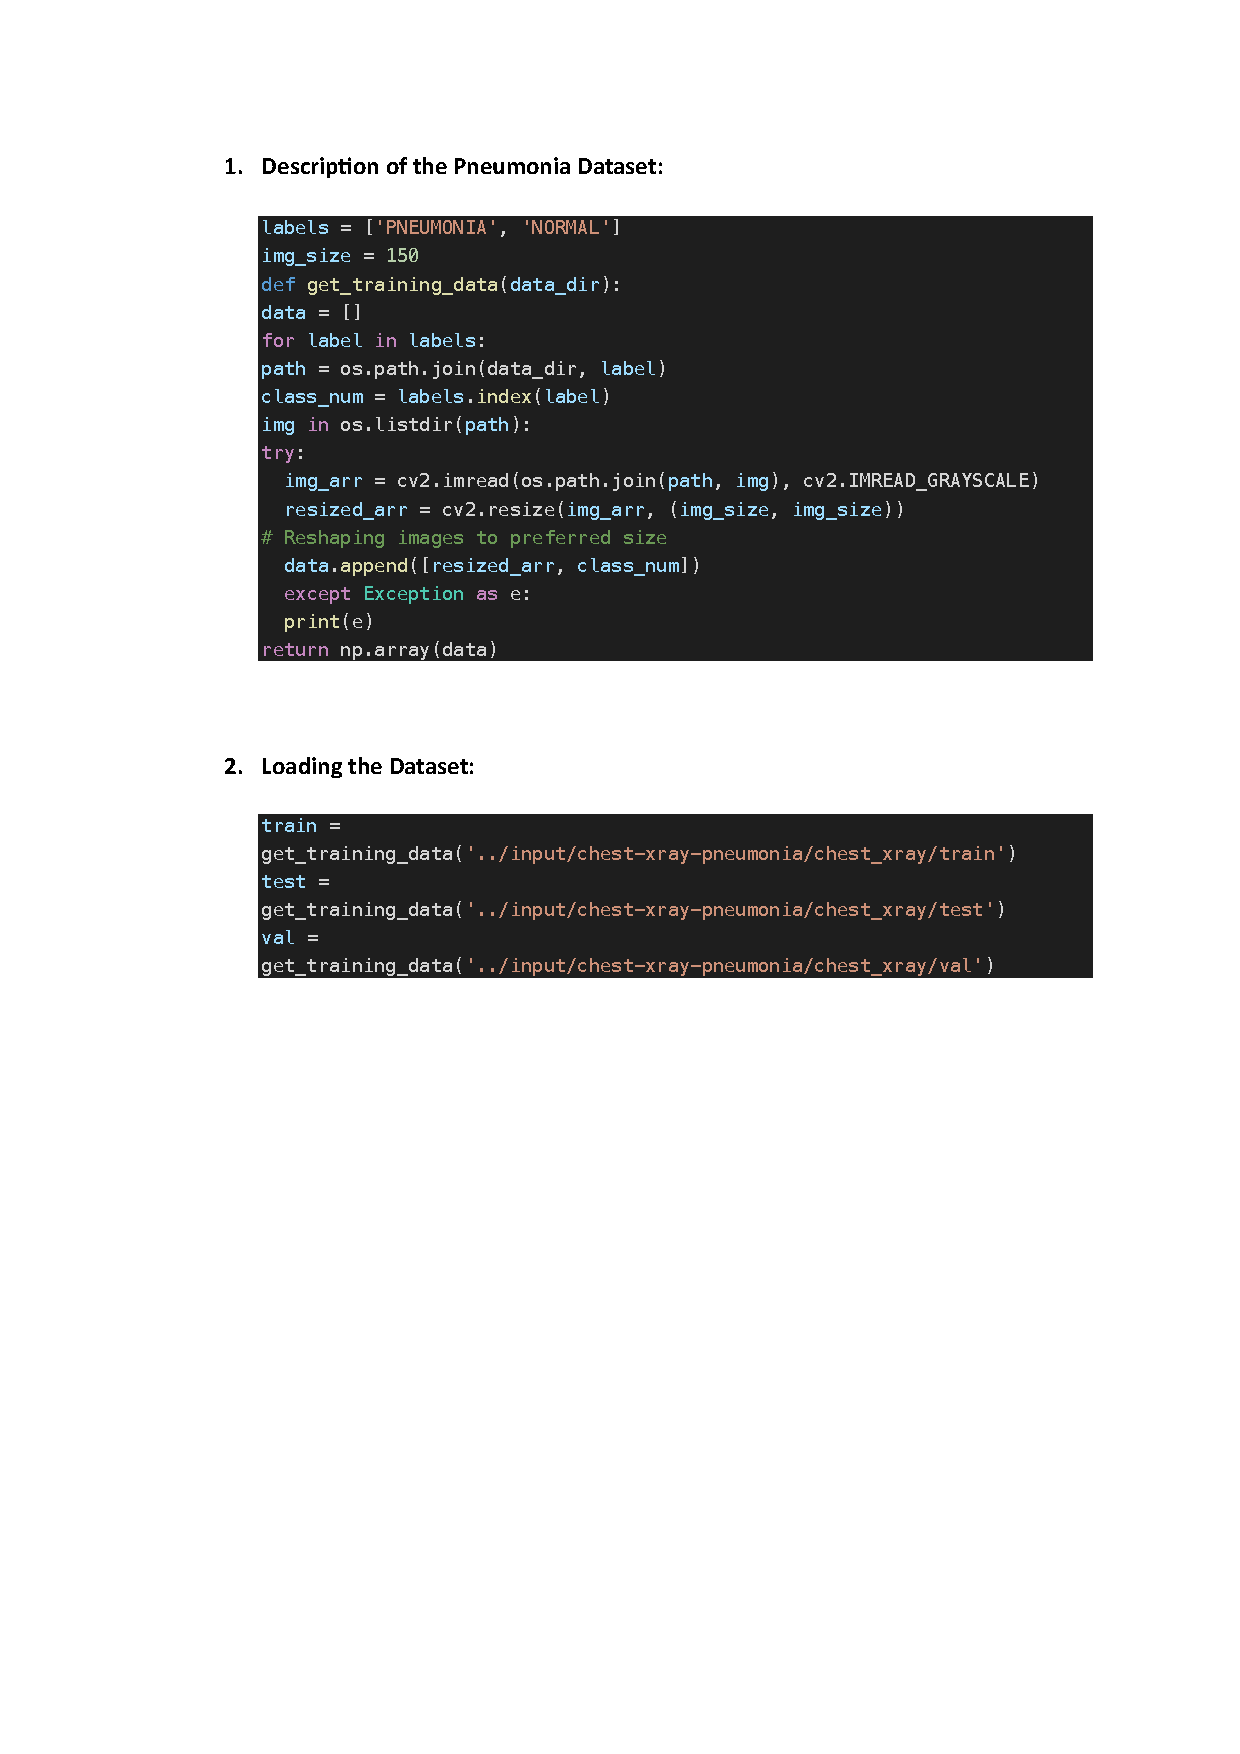
\includepdf[pages={-}]{Code/Data preparation.pdf}

 \bigskip
 
 \section{Data Preparation}
 
 In order to make data appropriate for analysis, data preparation is a crucial phase in the KDD methodology. It involves cleaning, filtering, converting, and integrating the data\cite{Witten:2002}. The data preparation procedures for the study to identify pneumonia using chest X-ray pictures are  the following:

 \bigskip
 \begin{enumerate}
 	
 	\item \textbf{Data collection:} The chest X-ray images were collected from the Guangzhou Women and Children’s Medical Center in Guangzhou.
 	\item \textbf{Data organization:} The dataset was organized into three folders (train, test, val) and further divided into subfolders for each image category (Pneumonia/Normal).
 	\item \textbf{Data cleaning:} The images were screened for quality control, and any low-quality or unreadable scans were removed.
 	\item \textbf{Data splitting:} The dataset was split into training, validation, and testing sets to evaluate the model's performance.

 \end{enumerate}

 
  \section{Data Transformation}
 
It involves retraining an InceptionV3 model that has already been trained using the provided dataset. The extensive ImageNet dataset, which includes millions of photos from numerous categories, served as the model's initial training ground. For the specific goal of identifying pneumonia from chest X-ray pictures, the model must be fine-tuned using the new dataset.\cite{Geron:2022}
  \bigskip
 
 The InceptionV3 model's output layers are eliminated during the transformation phase, and the top few layers are frozen to preserve the pre-trained weights. After training the model for the new label classes (Pneumonia and Normal), it is then fine-tuned using the new dataset. The model can learn characteristics relevant to the new dataset through the fine-tuning process while keeping the broad features it has already learnt from the ImageNet dataset.
 \bigskip
 
 In deep learning and transfer learning applications, this data transformation procedure is essential since it enables the pre-trained models to be modified for new tasks without requiring a significant amount of new data for training.
  \bigskip
  
  To avoid bias because of less pneumonia X-ray images, Data is augmentated to maintain the balance.
 \begin{enumerate}
 	
 	\item \textbf{Data Augmentation}
 	\lstinputlisting[language=Python]{Code/Data Augmentation.py}
 
 \end{enumerate}
 \bigskip
 
 \section{Data Mining}
 
 Data mining is the  technique of classifying chest X-ray pictures into two groups, Pneumonia or Normal, by utilizing a \ac{cnn}  to discover patterns and attributes.
  \bigskip
  
 A CNN is a kind of deep learning neural network created especially for processing and image identification. It is made up of several convolutional filter layers that have been trained to extract patterns and features from the input images. The classification operation is subsequently carried out by a fully linked layer using these features.
 \bigskip
 
 \subsection{Data Training}
 
 The CNN model was trained on the preprocessed data during the data mining stage of this research to discover the characteristics and patterns in the chest X-ray pictures that identify Pneumonia from Normal. By retraining an earlier InceptionV3 model that had been trained using millions of photos from the ImageNet database, the model was improved using transfer learning.
 \bigskip
 
 
 \lstinputlisting[language=Python]{Code/Training Model.py}
 
 The model was fed batches of images together with their associated labels during training, and the weights of the filters were changed iteratively to reduce the loss function. After the model had been trained, its accuracy, precision, and recall were assessed on a different set of test images.
 \bigskip
 
 
 The obtained CNN model  can classify chest X-ray images into two categories with a high degree of accuracy. This model can be used for real-world applications such as automated screening of chest X-rays for Pneumonia, enabling faster and more accurate diagnoses.
 \cite{Kermany:2018}
 
  
 \subsection{Transfer Learning}
 
 A pre-trained model on a sizable dataset is utilized as the basis for a new model for a related job in the transfer learning technique. In this scenario, a pre-trained CNN model, like InceptionV3, is utilized as a starting point and is then adjusted for the specific job of detecting pneumonia in chest X-ray pictures.\cite{Rajpurkar:2017} Transfer learning algorithm architecture can be seen in figure. 6.3.:\\
 \bigskip 
 
 \begin{figure}
 	\centering
 	\begin{tikzpicture}
 		\node at (0,0) {\includegraphics[width=\linewidth]{Images/Transfer Learning.png}};
 	\end{tikzpicture}
 	\caption{\textbf{Transfer learning architecture}}
 	\footnotesize \textbf{Reference:}\cite{Firdiantika:2022}
 		\label{fig:Transfer learning architecture}
 	\end{figure}
 	
 	Features like edges, corners, and curves are often detected by the lower layers of a pre-trained CNN, while objects and other forms are typically detected by the higher layers. It is possible to reuse the bottom layers of a pre-trained model to improving performance. On the new dataset, only the higher layers have been fine-tuned to learn the specific features required for the pneumonia detection task. \cite{ Rajpurkar:2018}
 	\bigskip   
 	
 	
 	
 	
 	

 
 
